\section{Transfer to image classification: More results and addition details}

\subsection{Linear probing with L-BFGS}\label{app:linear}
An alternative to doing linear probing with SGD is to use the convex optimization technique, L-BFGS~\citep{byrd1995limited}. It is very effective and has strict convergence guarantees. We compare SGD and L-BFGS for a variety of ViT models using the ImageNet-1k datasset. Specifically, we precompute image embeddings by resizing input images to 224px resolution and then solve the multiclass logistic regression problem with L-BFGS. We also sweep the L2 regularization parameter and select the optimal one using 20000 holdout images from the training data (approximately 2\% of the training data). In \cref{tab:app:bfgs} we compare the resulting model with the SGD baseline from the main text. It demonstrates that L-BFGS matches or lags behind SGD approach, so we selected the latter technique for our core experiments.

\begin{table}[h]
    \caption{Comparison of SGD and L-BFGS for linear probing on ImageNet-1k. The numbers indicate top-1 accuracy.}
\centering
\small
  \setlength{\tabcolsep}{4pt}
    \begin{tabular}{@{} l c c c c c c c @{}}
      \toprule
	    Linear Probing & B/32 & B/16 & L/16 & g/14 & G/14 & e/14 & 22B \\
      \midrule
      L-BFGS & 79.94 & 84.06 & 86.64 & 88.46 & 88.79 & 89.08 & 89.27 \\
      SGD & 80.18 & 84.20 & 86.66 & 88.51 & 88.98 & 89.26 & 89.51 \\
      \bottomrule
 \end{tabular}
    \label{tab:app:bfgs}
\end{table}


\label{app:image_classification}
% \subsubsection{Fine-tuning}
% \paragraph{Experimental setup.} We use the same fine-tuning recipe from~\citep{dosovitskiy2020image} on CIFAR-10, CIFAR-100, Oxford-IIIT Pet and Oxford Flowers. 
% We replace the original head parameters from the checkpoint before upstream cooldown with new parameters, initialized at zero. 
% The entire model is then finetuned on images with a resolution of 384px with mild random cropping and horizontal flipping.
% We use SGD with momentum ($\mu = 0.9$, batch size of 512).
% On CIFAR we train for 10\,000 steps with 500 warmup steps. On the Oxford datasets we train for 500 steps with 100 warmup steps.
% We tuned only the learning rate (over \{0.001, 0.003, 0.01 and 0.03\}) using the validation split of each dataset. 
% The only difference with respect to the fine-tuning recipe from~\citep{dosovitskiy2020image} is that we use mixup with $\alpha = 0.2$, and minimize the \emph{sigmoid} cross-entropy loss.

% \paragraph{Results.}
% \Cref{tab:standard4_ft} We showshows the fine-tuning accuracy on these datasets. 

% \begin{table}[t]
% \centering
% \caption{Fine-tuning accuracy on CIFAR-10, CIFAR-100, Oxford-IIIT Pet and Oxford Flowers.}
% \resizebox{\columnwidth}{!}{%
% \begin{tabular}{@{}l c c c c@{}}
% \toprule
% Model & C10 & C100 & Flower & Pet \\
% \midrule
% 22B   & 99.63} & 95.96 & 99.75} & 97.59} \\
% \midrule 
% L/16~\citep{dosovitskiy2020image} & 99.42 & 93.90 & 99.74 & 97.32 \\
% H/14~\citep{dosovitskiy2020image} & 99.50 & 94.55 & 99.68 & 97.56 \\
% EfficientNetV2-L~\citep{efficientnet_tan21} & 99.1\phantom{0} & 92.3\phantom{0} & 98.8\phantom{0} & -\\
% EffNet-L2+SAM~\citep{sam_foret2020} & - & 96.08} & 99.65 & 97.10 \\
% \bottomrule
% \end{tabular}
% }
% \label{tab:standard4_ft}
% \end{table}

% \subsection{Out-of-distribution}
% \label{app:robustness_ood}

\subsection{Out of distribution classification}
\label{app:ood}

\begin{table}[th]
    \caption{
        OOD Classification. Results from models fine-tuned on ImageNet (top half), and models that were only trained on JFT and evaluated with a label-map (bottom half).
        Models with ``ema'' are fine-tuned with Polyak averaging, similar to~\citep{dosovitskiy2020image}.
        B/16, L/16, g/14, and G/14 are from~\citep{zhai2022scaling}, and e/14 is from~\citep{chen2022pali}.
        IN$^\dagger$ uses same resize without crop like in the original publication.
        See \cref{fig:robustness_objectnet} and \cref{subsec:robustness_ood} for discussion of the results, and details about datasets and pre-processing.
    }
    \centering
    \setlength{\tabcolsep}{5pt}
    % \resizebox{\columnwidth}{!}{%
    \begin{tabular}{@{} l l c c c c c c @{}}
        \toprule
        % Model & Fine-tuned & IN & IN$_\square$ & INv2 & ObjectNet & IN-R & IN-A \\
        Model & Fine-tuned & IN & IN$^\dagger$ & INv2 & ObjectNet & IN-R & IN-A \\
        \midrule
        e/14 ema & 560px &   \textbf{90.70} & \textbf{90.84} &  84.38 &     72.53 & 94.49 & 88.44 \\
        22B ema & 560px &   90.62 &              - &  \textbf{84.65} &     \textbf{76.70} & \textbf{95.05} & \textbf{89.12} \\
        22B & 560px &   90.60 & - &  84.38 &     75.69 & 94.62 & 88.55 \\
        22B & 384px &   90.44 & - &  84.28 &     74.64 & 94.44 & 87.95 \\
        e/14 ema & 384px &   90.44 & - &  83.95 &     70.56 & 93.56 & 87.16 \\
        G/14 ema & 518px &   90.33 & 90.47 &  83.53 &     69.14 & 94.22 & 86.95 \\
        g/14 ema & 518px &   90.25 & 90.11 &  83.61 &     71.36 & 93.37 & 86.12 \\
        L/16 & 384px &   88.60 & - &  80.74 &     65.73 & 90.32 & 78.65 \\
        B/16 & 384px &   87.02 & - &  78.21 &     57.83 & 82.91 & 66.08 \\
        \midrule
        22B & - &    \textbf{78.5} & - &   \textbf{72.5} &      \textbf{66.9} &  \textbf{91.6} &  \textbf{79.9} \\
        e/14 & - &    76.7 & - &   71.0 &      64.4 &  90.6 &  75.3 \\
        G/14 & - &    76.6 & - &   70.9 &      63.3 &  90.2 &  75.1 \\
        g/14 & - &    76.3 & - &   70.5 &      62.6 &  89.8 &  73.7 \\
        L/16 & - &    73.9 & - &   66.9 &      58.4 &  86.8 &  64.6 \\
        B/16 & - &    70.7 & - &   62.9 &      52.9 &  81.4 &  51.1 \\
        \bottomrule
    \end{tabular}
    % }
    \label{tab:robustness_ood}
\end{table}


\subsection{Head2Toe}
The cost of fine-tuning a model during transfer learning goes up with increased model size and often requires the same level of resources as training the model itself. Linear probing on the other hand is much cheaper to run, however it often performs worse than fine-tuning. Recent work showed that training a linear classifier on top of the intermediate features can provide significant gains compared to using the last-layer only, especially for target tasks that are significantly different from the original pre-training task~\citep{evci22h2t,Adler2020CrossDomainFL, khalifa2022}. 

In \cref{tab:h2t_vtab} we compare Head2Toe~\citep{evci22h2t} with Linear probe on common vision benchmarks and VTAB-1k~\citep{zhai2019large}. We include Finetuning results as a comparison point. We use a simplified version of Head2Toe with no feature selection. Experimental details are shared below. Head2Toe achieves 7\% better results on VTAB-1k, however fails to match the full finetuning performance (-6\%). On other benchmarks (CIFARs, Flowers and Pets), all methods perform similarly potentially. Head2Toe improves over Linear only for the Cifar-100 task. For the remaining tasks it either achieves the same performance or worse (Pets).

% Rest is experimental details.  
All experiments presented here use images with the default resolution of 224. Head2Toe uses the following intermediate features: (1) output of each of the 48 blocks, (2) features after the positional embedding, (3) features after the pooling head (4) pre-logits and logits. We average each of these features among the token dimension and concatenate them; resulting in a 349081 dimensional feature vector. In contrast, linear probe uses the 6144 dimensional prelogit features, which makes Head2Toe training roughly 50 times more expensive. However, given the extraordinary size of the original model, Head2Toe requires significantly less FLOPs and memory\footnote{on the order of 1000x, the exact value depends on number of classes} compared to fine-tuning. For all tasks (4 standard and 19 VTAB-1k), we search over 2 learning rates (0.01, 0.001) and 2 training lengths (500 and 10000 (2500 for VTAB-1k) steps) using the validation set.

\begin{table}[htbp]
    \centering
    \caption{Frozen evaluation using linear and Head2Toe (H2T) probe on the VTAB-1k benchmark and four other image classification tasks. We report mean accuracies averaged using 3 seeds.}
    \label{tab:h2t_vtab}
    % \resizebox{0.8\columnwidth}{!}{%
    \begin{tabular}{@{}lrrrrrrrr@{}}
    \toprule
    Method &  VTAB-Average &  Natural & Specialized &  Structured &  CIFAR-10 & CIFAR-100 &   Flowers  &      Pets   \\
    \midrule
    Finetuning   & \textbf{76.71} &  \textbf{89.09} & 87.08 & \textbf{61.83} & \textbf{99.63} &    \textbf{95.96} & 97.59  &  \textbf{99.75}\\
    Linear   & 63.15 &  80.86 & 87.05 & 35.70 &  99.37 &    93.39 &  \textbf{99.75} &  98.15 \\
    H2T & 70.12 &  84.60 & \textbf{88.61} & 48.19 &  99.45 &  94.11 &  99.69 &  97.46 \\
    \bottomrule
    \end{tabular}
    % } %resizebox
%    \begin{tabular}{@{}lrrrr@{}}
%    \toprule
%    Method &  Average &  Natural & Specialized &  Structured   \\
%    \midrule
%    Finetuning   & 76.71 &  89.09 & 87.08 & 61.83 \\
%    Linear   & 63.15 &  80.86 & 87.05 & 35.70 \\
%    H2T & 70.12 &  84.60 & 88.61 & 48.19\\
%    \end{tabular}
%    % } %resizebox
%    \\
%    % \resizebox{0.8\columnwidth}{!}{%
%    \begin{tabular}{@{}lrrrr@{}}
%    \midrule
%     &  CIFAR-10 & CIFAR-100 &   Flowers  &      Pets \\
%
%    \midrule
%Finetuning       &  99.63 &    95.96 & 97.59  &  99.75 \\
%Linear       &  99.37 &    93.39 &  99.75 &  98.15 \\
%H2T      &  99.45 &  94.11 &  99.69 &  97.46 \\
%    \bottomrule
%    \end{tabular}
    % } %resizebox
%   \begin{tabular}{lrrrr}
%      &  IN-Real & IN-Val &   IN-v2 & IN-Tra \\
 
%     \midrule
% Linear   & 77.65 & 89.43 & 82.49 & 91.36 \\
% Head2Toe      & 76.68 & 87.82 & 79.37 & 89.95 \\
%     \end{tabular} 
\end{table}


\subsection{Few-shot}
We replicate the experimental setup of ~\citep{abnar2021exploring} to evaluate the \chonk model and baselines on 25 tasks (\cref{table:fewshot_datasets}) using few-shot transfer setups. The results of few-shot transfer of different models using 1, 5, 10, and 25 shots are presented in \cref{fig:fewshot}. 
Scaling up can improve performance in many tasks, but in some cases, downstream accuracy does not improve with increased scale. This may be due to the higher dimension of the representation from the \chonk model, which may require more regularization as the size of the head grows to prevent overfitting. Further study is needed to investigate this. 

\begin{figure*}[h]
    \centering
    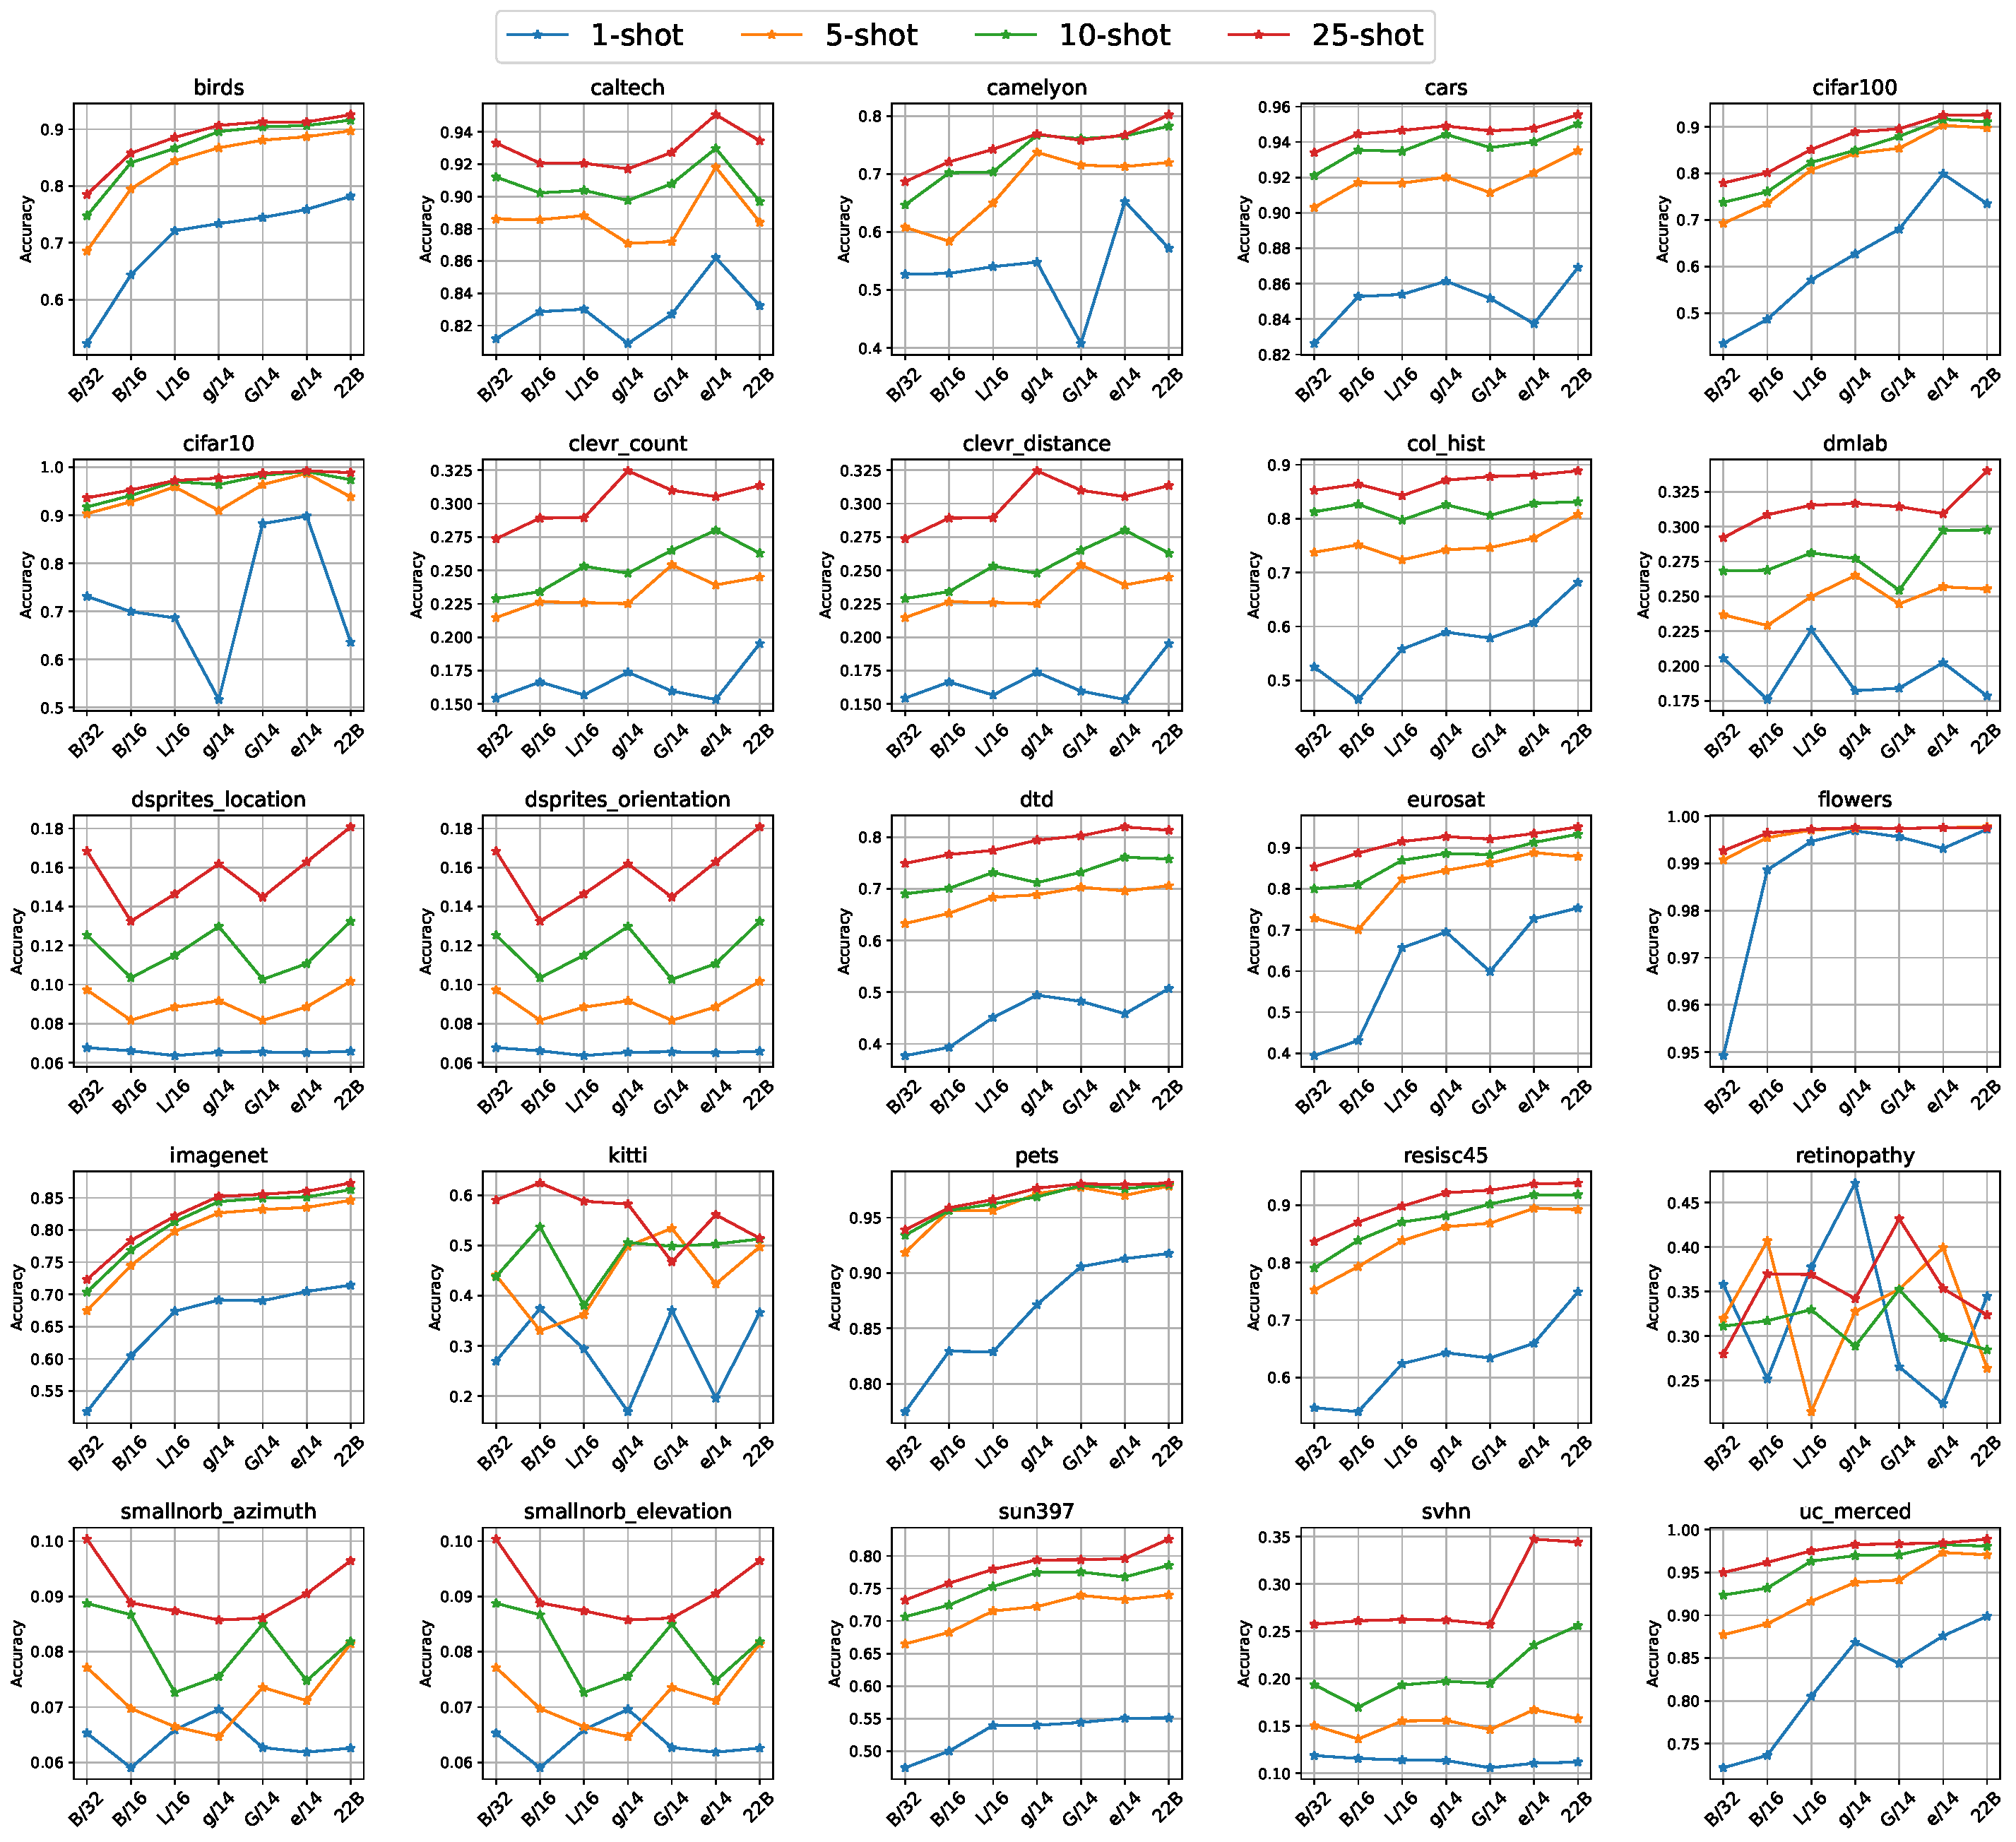
\includegraphics[width=0.95\columnwidth]{figs/fewshot_results.pdf}
    \vspace{-10pt}
    \caption{Few-shot transfer with 1, 5, 10, and 25 shots on 25 vision tasks~\citep{abnar2021exploring}.}
    \vspace{-15pt}
    \label{fig:fewshot}
\end{figure*}


\begin{table}[ht]
    \centering
    \caption{Summary of datasets used in our few-shot experiments in \cref{fig:fewshot}}
    {\fontsize{9}{9}\selectfont
    \resizebox{0.95\columnwidth}{!}{%
    \begin{tabular}{l p{12cm} p{5cm}}
     \textbf{Dataset}    & \textbf{Description} & \textbf{Reference} \\ \toprule
      ImageNet   & 1.28M labelled natural images. &~\citep{deng2009imagenet}\\ \midrule
      Caltech101 &The task consists in classifying pictures of objects (101 classes plus a background clutter class), including animals, airplanes, chairs, or scissors. The image size varies, but it typically ranges from 200-300 pixels per edge. &\citep{li_andreeto_ranzato_perona_2022} \\ \midrule
     CIFAR-10 & The task consists in classifying natural images (10 classes, with 6000 training images each). Some examples include apples, bottles, dinosaurs, and bicycles. The image size is 32x32.& \url{https://www.cs.toronto.edu/~kriz/cifar.html}\\ \midrule
      CIFAR-100 & The task consists in classifying natural images (100 classes, with 500 training images each). Some examples include apples, bottles, dinosaurs, and bicycles. The image size is 32x32.& \url{https://www.cs.toronto.edu/~kriz/cifar.html}\\ \midrule
      DTD & The task consists in classifying images of textural patterns (47 classes, with 120 training images each). Some of the textures are banded, bubbly, meshed, lined, or porous. The image size ranges between 300x300 and 640x640 pixels. &~\citep{cimpoi2014describing}\\ \midrule
      Pets & The task consists in classifying pictures of cat and dog breeds (37 classes with around 200 images each), including Persian cat, Chihuahua dog, English Setter dog, or Bengal cat. Images dimensions are typically 200 pixels or larger.& \url{https://www.robots.ox.ac.uk/~vgg/data/pets/} \\ \midrule
      Sun397 & The Sun397 task is a scenery benchmark with 397 classes and, at least, 100 images per class. Classes have a hierarchy structure and include cathedral, staircase, shelter, river, or archipelago. The images are (colour) 200x200 pixels or larger.& \url{https://vision.princeton.edu/projects/2010/SUN/}\\ \midrule
      Flowers102 & The task consists in classifying images of flowers present in the UK (102 classes, with between 40 and 248 training images per class). Azalea, Californian Poppy, Sunflower, or Petunia are some examples. Each image dimension has at least 500 pixels.& \url{https://www.robots.ox.ac.uk/~vgg/data/flowers/102/}\\ \midrule
      SVHN & This task consists in classifying images of Google’s street-view house numbers (10 classes, with more than 1000 training images each). The image size is 32x32 pixels.& \url{http://ufldl.stanford.edu/housenumbers/}\\ \midrule
      CLEVR/count & CLEVR is a visual question and answer dataset designed to evaluate algorithmic visual reasoning. We use just the images from this dataset, and create a synthetic task by setting the label equal to the number of objects in the images.& ~\citep{johnson2017clevr}\\ \midrule
      CLEVR/distance & Another synthetic task we create from CLEVR consists of predicting the depth of the closest object in the image from the camera. The depths are bucketed into size bins. &~\citep{johnson2017clevr}\\ \midrule
      Retinopathy & The Diabetic Retinopathy dataset consists of image-label pairs with high-resolution retina images, and labels that indicate the presence of Diabetic Retinopathy (DR) in a 0-4 scale (No DR, Mild, Moderate, Severe, or Proliferative DR). & \url{https://www.kaggle.com/c/diabetic-retinopathy-detection/data} \\ \midrule 
      Birds &  Image dataset with photos of 200 bird species (mostly North American). &~\citep{WahCUB_200_2011} \\ \midrule
      
      Patch Camelyon & The Patch Camelyon dataset contains 327,680 images of histopathologic scans of lymph node sections. The classification task consists in predicting the presence of metastatic tissue in given image (i.e., two classes). All images are 96x96 pixels. &~\citep{teh2019metric}\\ \midrule
      
        Resisc45 & The Remote Sensing Image Scene Classification (RESISC) dataset is a scene classification task from remote sensing images. There are 45 classes, containing 700 images each, including tennis court, ship, island, lake, parking lot, sparse residential, or stadium. The image size is RGB 256x256 pixels. &~\citep{cheng2017remote} \\ \midrule
        EuroSAT & The task consists in classifying Sentinel-2 satellite images into 10 different types of land use (Residential, Industrial, River, Highway, etc). The spatial resolution corresponds to 10 meters per pixel, and the image size is 64x64 pixels. &~\citep{helber2019eurosat} \\ \midrule
        dSprites/location & The dSprites dataset was originally designed to assess disentanglement properties of unsupervised learning algorithms. In particular, each image is a 2D shape where six factors are controlled: color, shape, scale, rotation, and (x,y) center coordinates. Images have 64x64 black-and-white pixels. This task consists in predicting the x (horizontal) coordinate of the object. The locations are bucketed into 16 bins & \url{https://github.com/deepmind/dsprites-dataset/}\\ \midrule
        dSprites/orientation & We create another task from dSprites consisting in predicting the orientation of each object, bucketed into 16 bins. & \url{https://github.com/deepmind/dsprites-dataset/https://github.com/deepmind/dsprites-dataset/} \\ \midrule
        SmallNORB/azimuth & The Small NORB dataset contains images of 3D-toys from 50 classes, including animals, human figures, airplanes, trucks, and cars. The image size is 640x480 pixels. In this case, we define labels depending on the azimuth (angle of horizontal deviation), in intervals of 20 degrees (18 classes). &~\citep{lecun2004learning}\\ \midrule
        SmallNORB/elevation & Another synthetic task we create from Small NORB consists in predicting the elevation in the image. There are 9 classes, corresponding to 9 different elevations ranging from 30 to 70 degrees, in intervals of 5 degrees & ~\citep{lecun2004learning} \\ \midrule
        DMLab & The DMLab (DeepMind Lab) is a set of control environments focused on 3D navigation and puzzle-solving tasks. The Dmlab dataset contains frames observed by the agent acting in the DeepMind Lab environment, which are annotated by the distance between the agent and various objects present in the environment. The goal is to evaluate the ability of a visual model to reason about distances from the visual input in 3D environments. The Dmlab dataset consists of 360x480 color images in 6 classes. The classes are {close, far, very far} × {positive reward, negative reward} respectively. &~\citep{beattie2016deepmind} \\ \midrule
        KITTI & The KITTI task consists in predicting the (binned) depth to the vehicle (car, van, or truck) in the image. There are 4 bins / classes. &~\citep{geiger2013vision}\\ \midrule
        ColHist & Classification of textures in colorectal cancer histology. Each example is a 150 x 150 x 3 RGB image of one of 8 classes. & \url{https://www.tensorflow.org/datasets/catalog/colorectal_histology} \\ \midrule
        UC Merced & 21 class land use image dataset & \url{https://usdahsi.ucmerced.edudatasets/landuse.html} \\
        \midrule
        Cars &  The Cars dataset contains 16,185 images of 196 classes of cars. The data is split into 8,144 training images and 8,041 testing images, where each class has been split roughly in a 50-50 split. Classes are typically at the level of Make, Model, Year, e.g. 2012 Tesla Model S or 2012 BMW M3 coupe.& \url{http://ai.stanford.edu/~jkrause/cars/car_dataset.html} \\ \bottomrule

    \end{tabular}
    }}
    \label{table:fewshot_datasets}
\end{table}

\clearpage
\newpage